\chapter{Metodologi Penelitian}

Bab ini menjelaskan langkah-langkah yang diambil dalam penelitian ini untuk mencapai tujuan yang ditetapkan dalam Subbab 1.3. Cakupannya meliputi alat dan bahan yang digunakan, metode penelitian, arsitektur sistem, alur data \textit{pipeline}, desain \textit{prompt} LLM, pemetaan kontrol ISO/IEC 27001:2022, rancangan eksperimen komparasi model, dan metode evaluasi.

\section{Alat dan Bahan Penelitian}

\subsection{Perangkat Keras}

Seluruh proses pengembangan dan pengujian dalam penelitian ini dilakukan pada satu unit laptop HP Victus 16-r0xxx dengan spesifikasi sebagai berikut:

\begin{itemize}
    \item Sistem operasi: Windows 11 Home Single Language 64-bit (Build 26200)
    \item Prosesor: Intel Core i7-13700HX, 24 inti logis, kecepatan dasar 2,1 GHz
    \item Memori: 16.384 MB RAM
    \item GPU diskrit: NVIDIA GeForce RTX 4060 dengan VRAM 8 GB
    \item GPU terintegrasi: Intel UHD Graphics
    \item Penyimpanan: NVMe SSD 1 TB
\end{itemize}

Alasan penggunaan spesifikasi ini bukan sekadar ketersediaan. Model LLM yang dijalankan secara lokal melalui Ollama membutuhkan VRAM yang cukup agar inferensi bisa berjalan sepenuhnya di GPU. RTX 4060 dengan VRAM 8 GB memungkinkan kelima model yang dievaluasi (masing-masing 6--8 miliar parameter) dijalankan pada kuantisasi Q4\_0 tanpa harus memindahkan sebagian perhitungan ke RAM atau CPU. Spesifikasi ini juga merepresentasikan perangkat keras kelas menengah yang realistis dimiliki oleh institusi atau pengembang individual, sehingga hasil pengujian tidak hanya berlaku di lingkungan riset yang ideal.

\subsection{Perangkat Lunak}

\begin{itemize}
    \item \textbf{Python 3.x}: Bahasa pemrograman utama untuk membangun \textit{pipeline} yang menghubungkan semua modul. Dipilih karena kemudahannya memanggil perintah eksternal via \textit{subprocess} dan ketersediaan pustaka \texttt{requests} untuk berkomunikasi dengan API Ollama.
    \item \textbf{Rector} \cite{rector2024}: Alat transformasi kode berbasis AST untuk PHP, dikonfigurasi secara dinamis sesuai versi target yang dipilih.
    \item \textbf{Semgrep} \cite{semgrep2024}: Alat analisis statis untuk pemindaian kerentanan. Dijalankan dengan \textit{ruleset} \texttt{p/php} dan \texttt{p/owasp-top-ten} \cite{owasp2021}.
    \item \textbf{PHPStan} \cite{phpstan2024}: Alat analisis statis untuk validasi tipe dan kompatibilitas kode PHP, dijalankan pada level 5.
    \item \textbf{Ollama} \cite{ollama2024}: \textit{Platform} untuk menjalankan LLM secara lokal, diakses via API REST di \texttt{localhost:11434}.
    \item \textbf{PHP 8.5.1}: Interpreter PHP untuk validasi sintaks menggunakan \texttt{php -l}.
    \item \textbf{Composer}: Manajer dependensi PHP untuk instalasi Rector dan PHPStan.
    \item \textbf{Visual Studio Code} dengan ekstensi Claude Code sebgai IDE utama selama pengembangan.
\end{itemize}

\subsection{Model LLM yang Dievaluasi}

Lima model LLM \textit{open source} dievaluasi, semuanya dijalankan secara lokal melalui Ollama tanpa \textit{fine-tuning}. Dua kriteria pemilihan diterapkan: model harus bisa dijalankan di GPU VRAM 8 GB pada kuantisasi Q4\_0, dan kemampuan pemahaman kodenya harus terdokumentasi dalam literatur ilmiah.

\begin{itemize}
    \item DeepSeek Coder 6.7b \cite{deepseek2024coder}: Model spesialis kode, dilatih pada 2 triliun token dengan 87\% kode sumber.
    \item Qwen2.5-Coder 7b \cite{hui2024qwen} \text:{} Model kode dari Alibaba, dilatih pada 5,5 triliun token kode.
    \item CodeLlama 7b \cite{roziere2024codellama}: Model berbasis Llama 2 dari Meta AI untuk tugas pemrograman.
    \item Mistral 7b \cite{jiang2023mistral}: Model tujuan umum dari Mistral AI dengan arsitektur \textit{grouped-query attention}.
    \item Llama 3.1 8b \cite{dubey2024llama3}: Model dari seri Llama 3 yang dilatih pada lebih dari 15 triliun token multibahasa.
\end{itemize}

\subsection{Bahan Penelitian}

\begin{itemize}
    \item \textbf{Dokumen ISO/IEC 27001:2022} \cite{iso27001_2022}: Acuan utama untuk pemetaan kontrol keamanan.
    \item \textbf{Kode sumber PHP dari DTI UGM}: Kumpulan \textit{file} PHP dari aplikasi web internal berbasis CodeIgniter 3.x. Bersifat rahasia dan hanya digunakan untuk analisis statis tanpa akses ke basis data produksi.
    \item \textbf{Dokumentasi resmi PHP} \cite{phpgroup2022supported}: Referensi untuk memverifikasi kebenaran konversi Rector.
    \item \textbf{Registri aturan Semgrep} \cite{semgrep2024}: Aturan publik \texttt{p/php} dan \texttt{p/owasp-top-ten} untuk pemindaian keamanan.
\end{itemize}

\section{Metode Penelitian}

Penelitian ini menggunakan metodologi Penelitian dan Pengembangan (\textit{Research and Development}, R\&D) dengan model prototipe. Pilihan ini didasarkan pada fakta bahwa penelitian menghasilkan produk perangkat lunak nyata, bukan hanya analisis teoritis. Model prototipe dipilih karena dalam praktiknya banyak keputusan desain baru bisa dibuat setelah melihat perilaku nyata sistem, bukan dari perencanaan di atas kertas saja. Ini terutama berlaku untuk format \textit{prompt} AI dan cara menangani kode yang tidak bisa diotomatisasi sepenuhnya.

Gambar \ref{fig:alur-penelitian} menunjukkan alur penelitian yang terdiri dari tujuh tahapan.

\begin{figure}[h]
    \centering
    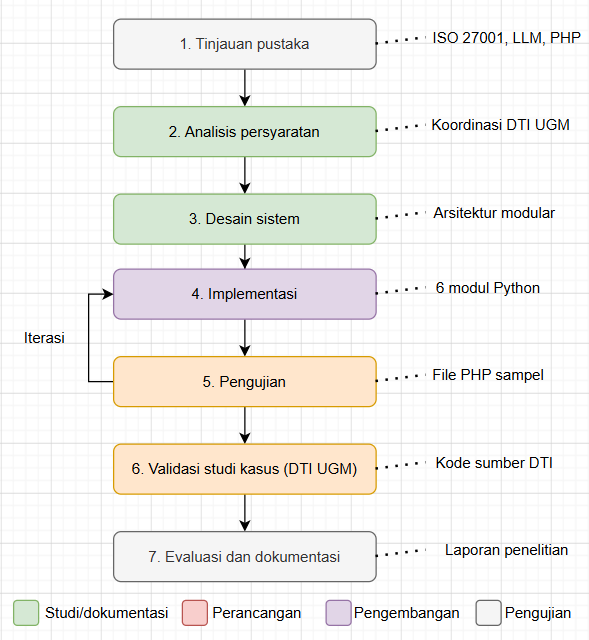
\includegraphics[width=0.7\textwidth]{contents/chapter-3/alur-penelitian.png}
    \caption{Alur penelitian dengan model prototipe}
    \label{fig:alur-penelitian}
\end{figure}

\begin{enumerate}
    \item \textbf{Tinjauan pustaka}: Mempelajari permasalahan migrasi PHP lama, persyaratan ISO/IEC 27001:2022 \cite{iso27001_2022}, kemampuan model LLM \textit{open source}, dan alat analisis statis yang relevan. Koordinasi awal dengan DTI UGM dilakukan pada tahap ini.
    \item \textbf{Analisis persyaratan}: Mendefinisikan persyaratan fungsional dan non-fungsional berdasarkan hasil tinjauan pustaka dan koordinasi dengan DTI UGM, termasuk menentukan kontrol ISO yang dicakup dan persyaratan privasi data.
    \item \textbf{Desain sistem}: Merancang arsitektur \textit{pipeline} secara modular dan menentukan tanggung jawab setiap modul.
    \item \textbf{Implementasi}: Membangun keenam modul Python satu per satu. Setiap modul diuji secara terpisah sebelum diintegrasikan.
    \item \textbf{Pengujian}: Menguji prototipe dengan \textit{file} PHP sampel. Jika ditemukan masalah, proses kembali ke tahap implementasi (iterasi).
    \item \textbf{Validasi studi kasus}: Pengujian akhir menggunakan kode sumber asli DTI UGM setelah prototipe stabil.
    \item \textbf{Evaluasi dan dokumentasi}: Menganalisis hasil dan menyusun laporan penelitian.
\end{enumerate}

\section{Arsitektur Sistem}

Sistem terdiri dari enam modul Python yang masing-masing menangani satu langkah dalam proses konversi dan analisis keamanan. \texttt{main.py} bertindak sebagai orkestrator yang mengontrol urutan eksekusi dan mengalirkan data antar modul. Arsitektur modular memungkinkan setiap bagian diuji, diperbaiki, atau diganti secara independen.

Gambar \ref{fig:arsitektur-sistem} menunjukkan hubungan antar modul.

\begin{figure}[h]
    \centering
    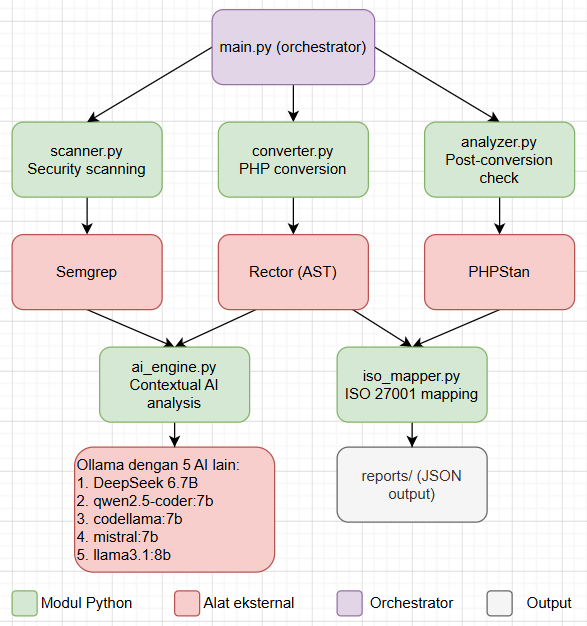
\includegraphics[width=0.7\textwidth]{contents/chapter-3/arsitektur-sistem.png}
    \caption{Arsitektur sistem \textit{pipeline} dengan enam modul Python}
    \label{fig:arsitektur-sistem}
\end{figure}

\subsection{Scanner (scanner.py)}

Modul pertama yang berjalan. Scanner menjalankan Semgrep \cite{semgrep2024} pada direktori \texttt{input/} sebelum konversi dimulai untuk menetapkan \textit{baseline} keamanan kode asli. Hasil pemindaian dikelompokkan berdasarkan jenis kerentanan (injeksi SQL, XSS, \textit{path traversal}, injeksi perintah, fungsi usang, kriptografi lemah) dan diberi tingkat prioritas. Data ini menjadi pembanding untuk mengukur perubahan keamanan setelah konversi.

\subsection{Converter (converter.py)}

Modul ini menggunakan Rector \cite{rector2024} untuk transformasi kode PHP berbasis AST. Argumen CLI \texttt{--target-php} menentukan versi target; nilai yang diterima adalah \texttt{"7.4"}, \texttt{"8.0"}, \texttt{"8.1"}, \texttt{"8.2"}, atau \texttt{"8.3"}. Sebelum Rector dijalankan, seluruh \textit{file} PHP dari \texttt{input/} disalin dahulu ke \texttt{output/}. Rector kemudian memodifikasi \textit{file} di \texttt{output/} di tempat. \textit{File} yang gagal dikonversi tetap ada di \texttt{output/} sebagai salinan kode asli dan statusnya dicatat \texttt{FAILED} di laporan; direktori \texttt{input/} tidak pernah disentuh. Konfigurasi Rector dibuat sebagai \textit{tempfile} saat \textit{runtime} dan dihapus otomatis setelahnya.

\begin{table}[h]
\centering
\caption{Pemetaan argumen \texttt{--target-php} ke konfigurasi Rector}
\label{tab:rector-levelset}
\begin{tabularx}{\textwidth}{|l|X|X|}
\hline
\textbf{Nilai \texttt{--target-php}} & \textbf{LevelSetList yang diterapkan} & \textbf{Cakupan rule kumulatif} \\
\hline
\texttt{7.4} & \texttt{UP\_TO\_PHP\_74} & PHP 5.2, 5.3, 5.4, 5.5, 5.6, 7.0, 7.1, 7.2, 7.3, 7.4 \\
\hline
\texttt{8.0} & \texttt{UP\_TO\_PHP\_80} & Semua rule 7.4 + PHP 8.0 \\
\hline
\texttt{8.1} & \texttt{UP\_TO\_PHP\_81} & Semua rule 8.0 + PHP 8.1 \\
\hline
\texttt{8.2} & \texttt{UP\_TO\_PHP\_82} & Semua rule 8.1 + PHP 8.2 \\
\hline
\texttt{8.3} & \texttt{UP\_TO\_PHP\_83} & Semua rule 8.2 + PHP 8.3 \\
\hline
\end{tabularx}
\end{table}

Karena \textit{ruleset}-nya kumulatif, kode PHP 5.x pun bisa diproses langsung menuju PHP 8.3 dalam satu langkah. Transformasi seperti \texttt{var} menjadi \texttt{public}, \texttt{array()} menjadi \texttt{[]}, dan penghapusan modifier \texttt{/e} pada \texttt{preg\_replace()} ditangani sepenuhnya. Yang tidak bisa ditangani adalah \texttt{mysql\_*()} karena butuh penulisan ulang semantik, bukan sekadar penggantian sintaks.

\subsection{Analyzer (analyzer.py)}

Setelah konversi, Analyzer menjalankan PHPStan \cite{phpstan2024} pada direktori \texttt{output/} untuk memverifikasi kompatibilitas kode dengan versi PHP target. Level 5 dipilih sebagai keseimbangan antara keketatan dan jumlah \textit{false positive} yang wajar untuk kode warisan. Setiap temuan PHPStan dikategorikan sebagai ERROR atau WARNING, lalu dikaitkan dengan kontrol ISO/IEC 27001:2022 yang relevan.

\subsection{AI Engine (ai\_engine.py)}

Modul ini menerima temuan dari Semgrep \textit{pre-scan} sebagai masukan, bukan dari PHPStan dan bukan dari \textit{post-scan}. Hanya temuan dengan prioritas 1--3 yang dikirim ke AI Engine: SQL Injection (prioritas 1), XSS (prioritas 2), dan fungsi usang (prioritas 3). Temuan prioritas 4 ke atas seperti \textit{hardcoded credentials} dan \textit{path traversal} tidak diproses.

Untuk setiap temuan yang lolos filter, modul mengirimkan konteks dan potongan kode ke model LLM melalui endpoint \texttt{/api/chat} Ollama \cite{ollama2024} di \texttt{localhost:11434}. Kalau model tidak menghasilkan blok kode PHP sama sekali, respons tetap dicatat dengan \textit{placeholder} \texttt{// Manual review required}, bukan di-skip. Jika Ollama tidak tersedia, \textit{pipeline} tetap berjalan tanpa komponen AI. Desain \textit{prompt} yang digunakan dibahas dalam Subbab \ref{sec:prompt-design}.

\subsection{ISO Mapper (iso\_mapper.py)}

Modul ini menerima semua hasil dari Scanner, Analyzer, dan AI Engine sebagai objek Python \textit{in-memory} langsung dari \texttt{main.py}, lalu memetakannya ke kontrol ISO/IEC 27001:2022 \cite{iso27001_2022} secara berbasis aturan. Tidak ada pembacaan \textit{file} JSON. Pemetaan berbasis aturan dipilih agar hasilnya deterministik dan dapat diaudit. Detail pemetaan dibahas dalam Subbab \ref{sec:iso-mapping-design}.

\subsection{Main (main.py)}

Orkestrator yang mengontrol seluruh \textit{pipeline}. Menerima direktori \textit{input} dan versi PHP target sebagai argumen CLI, menjalankan kelima modul secara berurutan, dan menghasilkan laporan JSON di direktori \texttt{reports/}. Ringkasan hasil ditampilkan di konsol menggunakan pustaka Rich.
\newpage
\section{Alur Data Pipeline}

Gambar \ref{fig:alur-pipeline} menunjukkan alur data lengkap dari masukan hingga laporan akhir.

\begin{figure}[h]
    \centering
    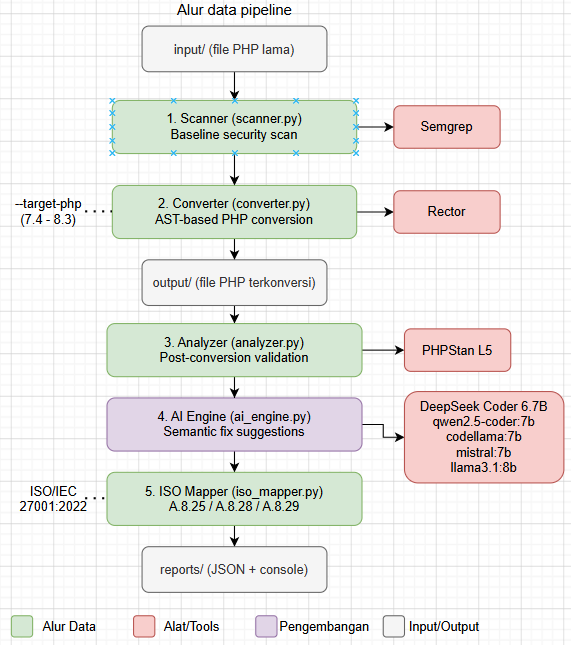
\includegraphics[width=0.8\textwidth]{contents/chapter-3/alur-data-pipeline.png}
    \caption{Alur data \textit{pipeline} dari \textit{input} hingga laporan akhir}
    \label{fig:alur-pipeline}
\end{figure}

Alurnya cukup linear. \textit{File} PHP ditempatkan di \texttt{input/}. Scanner memindai dengan Semgrep untuk menetapkan \textit{baseline}. Converter menyalin semua \textit{file} ke \texttt{output/} lalu menjalankan Rector dengan versi target yang ditentukan; \texttt{input/} tidak tersentuh. Analyzer menjalankan PHPStan level 5 pada \texttt{output/}. AI Engine mengambil temuan Semgrep prioritas 1--3 dan mengirimkannya ke model LLM. ISO Mapper mengumpulkan semua temuan dan memetakannya ke kontrol ISO. \texttt{main.py} menggabungkan semuanya menjadi laporan JSON dan menampilkan ringkasan di konsol.

\section{Desain Prompt LLM}
\label{sec:prompt-design}

Desain \textit{prompt} adalah salah satu keputusan metodologis yang paling berpengaruh terhadap kualitas respons model. Tiga tujuan harus dipenuhi sekaligus: mendapatkan kode perbaikan yang valid sintaksisnya, mendapatkan skor kepercayaan yang bisa di-\textit{parse} otomatis oleh \textit{pipeline}, dan bisa dijalankan \textit{zero-shot} tanpa contoh karena tidak ada \textit{dataset} berlabel yang tersedia.

\subsection{Struktur Prompt}

\textit{Prompt} terdiri dari dua bagian yang dikirim melalui endpoint \texttt{/api/chat}: \textit{system message} dan \textit{user message}. \textit{System message}:

\begin{verbatim}
You are a PHP security expert and migration specialist. You analyze
PHP code for security vulnerabilities and provide secure PHP 8.x
replacements. Always follow output format instructions exactly as
given.
\end{verbatim}

\textit{User message} untuk setiap temuan:

\begin{verbatim}
TASK: Analyze the following PHP code for a [vulnerability_type]
vulnerability and provide a secure PHP 8.x replacement.
ISO/IEC 27001:2022 Controls: [relevant_controls]
Context: File: [filename], line [line_number],
         Semgrep rule: [rule_id], Finding: [description]

VULNERABLE CODE:
```php
[code_snippet]
```

Respond in English:
1. Explain the vulnerability and its security risk.
2. Provide the corrected PHP 8.x code in a ```php code block.

After your explanation and code fix, write exactly this on the
last line:
CONFIDENCE: [number between 0 and 100]

Example last line: CONFIDENCE: 85
\end{verbatim}

\subsection{Keputusan Desain Prompt}

\textbf{Penyertaan kontrol ISO/IEC 27001:2022.} Kontrol ISO yang relevan disertakan di setiap \textit{prompt}. Ini bukan konteks dekoratif; tujuannya mendorong model menghasilkan saran perbaikan yang mempertimbangkan kepatuhan standar, bukan sekadar memperbaiki sintaks.

\textbf{Instruksi format di akhir pesan.} Format \texttt{CONFIDENCE: [0-100]} diletakkan di bagian akhir dengan instruksi eksplisit termasuk contoh konkret. Model kecil cenderung lebih patuh pada instruksi yang dekat dengan akhir pesan.

\textbf{Parsing skor berlapis.} Karena tidak semua model mengikuti format yang diminta, \texttt{ai\_engine.py} menggunakan enam pola \textit{regex} berurutan untuk mengekstraksi skor: (0) tag XML \texttt{<confidence>}, (1) bilangan bulat dekat kata "confidence", (2) desimal 0.x dekat "confidence", (3) persentase dekat "confidence", (4) desimal \textit{bare} di mana saja, dan (5) frasa bahasa alami seperti "not sure" yang dipetakan ke nilai tetap. Jika semua gagal, dikembalikan nilai \textit{default} 0,0.

\textbf{Temperature 0,1.} Dipilih untuk meminimalkan variasi acak antar percobaan. Setiap model dijalankan tiga kali per temuan dengan \textit{prompt} identik, sehingga perbedaan hasil antar \textit{run} mencerminkan variabilitas model yang sebenarnya.

\textbf{Zero-shot tanpa contoh.} Tidak ada contoh perbaikan kode disertakan karena penelitian ingin mengevaluasi kemampuan bawaan model dalam kondisi yang merepresentasikan penggunaan nyata. Ini juga memastikan semua model dibandingkan pada kondisi yang setara.

\textbf{Skor kepercayaan sebagai metrik sekunder.} Skor ini adalah penilaian mandiri dari model dan tidak bisa diverifikasi secara independen. Dalam analisis Bab IV, skor kepercayaan adalah metrik sekunder; metrik primer adalah validitas sintaks kode yang dihasilkan, diukur dengan \texttt{php -l}.

\section{Desain Pemetaan ISO/IEC 27001:2022}
\label{sec:iso-mapping-design}

Pemetaan temuan ke kontrol ISO/IEC 27001:2022 dilakukan secara berbasis aturan di dalam \texttt{iso\_mapper.py}. Data diterima langsung sebagai objek Python \textit{in-memory} dari \texttt{main.py}, tidak dibaca dari \textit{file} JSON. Pilihan desain berbasis aturan ini disengaja agar hasilnya deterministik dan bisa diaudit, berbeda dari pendekatan berbasis AI yang hasilnya bisa berubah antar inferensi. Ada enam kontrol yang dipetakan, sebagaimana ditunjukkan pada Tabel \ref{tab:iso-mapping}.

\begin{table}[h]
\centering
\caption{Pemetaan sumber temuan ke kontrol ISO/IEC 27001:2022 Annex A}
\label{tab:iso-mapping}
\begin{tabularx}{\textwidth}{|l|l|X|}
\hline
\textbf{Kontrol ISO} & \textbf{Judul} & \textbf{Sumber temuan yang dipetakan} \\
\hline
A.5.17 & \textit{Authentication Information} & Semgrep: \textit{hardcoded credentials} \\
\hline
A.8.24 & \textit{Use of Cryptography} & Semgrep: \texttt{md5()}/\texttt{sha1()} untuk kata sandi \\
\hline
A.8.25 & \textit{Secure Development Lifecycle} & Semgrep (semua) + PHPStan ERROR/WARNING \\
\hline
A.8.26 & \textit{Application Security Requirements} & Semgrep: SQL Injection, XSS \\
\hline
A.8.28 & \textit{Secure Coding} & Semgrep (semua) + PHPStan ERROR \\
\hline
A.8.29 & \textit{Security Testing in Development} & PHPStan ERROR/WARNING \\
\hline
\end{tabularx}
\end{table}

Status akhir setiap kontrol ditentukan berdasarkan ada tidaknya temuan terbuka setelah \textit{pipeline} selesai. \texttt{COMPLIANT} berarti tidak ada temuan yang dipetakan ke kontrol tersebut. \texttt{NON\_COMPLIANT} berarti ada temuan Semgrep aktif. \texttt{PARTIAL} berarti hanya ada temuan PHPStan tanpa temuan Semgrep. Perlu dicatat bahwa \texttt{COMPLIANT} pada A.5.17 dan A.8.24 bukan berarti kode bebas masalah secara absolut, melainkan \textit{ruleset} yang digunakan tidak menghasilkan temuan yang dipetakan ke kedua kontrol itu pada dataset ini.

\section{Dataset Studi Kasus}

Studi kasus menggunakan 245 \textit{file} PHP dari satu aplikasi web internal berbasis CodeIgniter 3.x yang dikelola oleh DTI UGM. Struktur direktorinya mengikuti konvensi standar CodeIgniter 3.x: \texttt{application/} untuk kode aplikasi (kontroler, model, \textit{view}, \textit{helper}, konfigurasi, layanan) dan \texttt{system/} untuk kode \textit{framework}. Kode diperoleh melalui koordinasi langsung dengan DTI UGM dan hanya digunakan untuk analisis statis dalam lingkungan lokal, tanpa akses ke basis data produksi dan tanpa eksekusi kode.

Hanya \textit{file} \texttt{.php} yang diproses; \textit{file} lain seperti \texttt{.html}, \texttt{.js}, dan \texttt{.css} tidak disalin ke \texttt{output/} dan tidak dianalisis. Dataset mencerminkan karakteristik kode warisan yang umum: pencampuran logika bisnis, akses basis data, dan presentasi dalam \textit{file} yang sama, serta beberapa pola kode PHP 5.x yang masih ada meski aplikasi secara keseluruhan berjalan di atas PHP 7.x.

Untuk eksperimen komparasi LLM, digunakan 11 temuan dari Semgrep \textit{pre-scan}: 1 SQL Injection dan 10 SSRF (\textit{Server-Side Request Forgery}). Ini adalah seluruh populasi temuan \textit{pre-scan}, bukan subset yang dipilih secara subjektif.

\section{Rancangan Eksperimen Komparasi Model LLM}

Eksperimen komparasi dirancang dengan kondisi yang sepenuhnya terkontrol dan dilakukan terpisah dari pengujian \textit{pipeline} utama menggunakan skrip evaluasi khusus.

\subsection{Kondisi Eksperimen}

\begin{itemize}
    \item \textbf{Input}: 11 temuan Semgrep dari \textit{pre-scan} dataset DTI UGM
    \item \textbf{Jumlah percobaan}: 3 \textit{run} per temuan per model (33 percobaan per model, 165 total)
    \item \textbf{Temperature}: 0,1 untuk semua model
    \item \textbf{Prompt}: identik untuk semua model dan semua percobaan (\textit{zero-shot})
    \item \textbf{Model}: dijalankan lokal melalui Ollama tanpa modifikasi
\end{itemize}

\subsection{Metrik Evaluasi}

\textbf{Format compliance rate} mengukur persentase respons yang mengikuti format \textit{prompt} yang diminta. Sebuah respons dianggap patuh jika mengandung blok kode PHP yang bisa diekstraksi, penjelasan bahasa alami, dan skor kepercayaan dalam format \texttt{CONFIDENCE: [0-100]}. Diukur otomatis oleh skrip \texttt{llm\_comparison.py}. Metrik ini mencerminkan kemampuan model mengikuti instruksi, bukan kualitas kodenya.

\textbf{Syntax validity rate} mengukur persentase blok kode PHP yang diekstraksi dari respons dan lolos \texttt{php -l}. Diukur oleh \texttt{llm\_quality\_checker.py} secara objektif. Ini adalah metrik primer karena hasilnya konkret dan bisa diverifikasi secara independen. \textit{Format compliance rate} adalah metrik sekunder.

\subsection{Interpretasi Trade-off Antar Metrik}

Kedua metrik bisa memberikan gambaran yang berbeda dan perlu diinterpretasikan hati-hati. Model yang patuh format tapi menghasilkan kode bermasalah secara sintaksis menunjukkan kemampuan mengikuti instruksi tapi kualitas kode rendah. Sebaliknya, model dengan kepatuhan format rendah tapi validitas sintaks tinggi menunjukkan model mengabaikan format instruksi namun kode yang berhasil diekstraksi berkualitas baik. Kedua kondisi ini punya implikasi praktis yang berbeda dan akan dibahas di Bab IV.

\section{Keamanan dan Privasi Data}

Kode PHP dari DTI UGM adalah aset institusi yang tidak boleh dikirimkan ke layanan eksternal. Kendala inilah yang menentukan arsitektur AI dalam penelitian ini. Daripada menggunakan API LLM berbasis \textit{cloud}, penelitian ini menggunakan Ollama \cite{ollama2024} sebagai \textit{runtime} lokal sehingga seluruh inferensi terjadi di mesin pengembangan.

Tidak ada data yang dikirimkan ke \textit{server} eksternal. Seluruh proses analisis berlangsung secara statis: tidak ada koneksi ke basis data produksi DTI UGM, tidak ada eksekusi kode PHP. Keputusan ini sejalan dengan ISO/IEC 27001:2022 \cite{iso27001_2022} yang mensyaratkan pemisahan lingkungan pengembangan dan pengendalian akses terhadap aset informasi sensitif.

\section{Metode Pengujian dan Evaluasi}

Pengujian dilakukan dengan pendekatan \textit{black-box}, fokus pada \textit{output} setiap modul bukan detail implementasi internal. Ada lima metrik utama:

\begin{enumerate}
    \item \textbf{Tingkat konversi Rector}: Persentase \textit{file} PHP yang berhasil dikonversi tanpa kesalahan fatal Rector, dihitung per \textit{file} dan secara keseluruhan.

    \item \textbf{Validitas sintaks pasca-konversi}: Persentase \textit{file} hasil konversi yang lolos \texttt{php -l}. Diukur secara objektif.

    \item \textbf{Perbedaan temuan keamanan}: Selisih jumlah temuan Semgrep antara \textit{pre-scan} dan \textit{post-scan}. Temuan baru setelah konversi tidak otomatis diinterpretasikan sebagai regresi keamanan; bisa jadi merupakan kerentanan laten yang sebelumnya tersembunyi dan baru terlihat setelah transformasi kode.

    \item \textbf{Performa model LLM}: Diukur menggunakan \textit{format compliance rate} (sekunder) dan \textit{syntax validity rate} (primer) sebagaimana dijelaskan dalam Subbab 3.8.

    \item \textbf{Status kepatuhan ISO/IEC 27001:2022}: Status per kontrol (\texttt{COMPLIANT}, \texttt{PARTIAL}, atau \texttt{NON\_COMPLIANT}) berdasarkan logika pemetaan dalam Subbab \ref{sec:iso-mapping-design}.
\end{enumerate}

Untuk hasil PHPStan, jumlah kesalahan yang tinggi tidak langsung diinterpretasikan sebagai kegagalan \textit{pipeline}. Kesalahan PHPStan pada kode warisan yang baru dimigrasi sebagian besar mencerminkan \textit{technical debt} yang sudah ada sebelum migrasi, bukan akibat dari proses konversi. Pembedaan ini dibahas lebih rinci di Bab IV.